\documentclass[conference]{IEEEtran}

%\usepackage{cite}

% *** GRAPHICS RELATED PACKAGES ***
%
\ifCLASSINFOpdf
  %\usepackage[pdftex]{graphicx}
  \usepackage[demo]{graphicx}
  % declare the path(s) where your graphic files are
  \graphicspath{{./fig/}}
  % and their extensions so you won't have to specify these with
  % every instance of \includegraphics
  \DeclareGraphicsExtensions{.pdf,.jpeg,.png}
\else
  % or other class option (dvipsone, dvipdf, if not using dvips). graphicx
  % will default to the driver specified in the system graphics.cfg if no
  % driver is specified.
  \usepackage[dvips]{graphicx}
  % declare the path(s) where your graphic files are
  % \graphicspath{{../eps/}}
  % and their extensions so you won't have to specify these with
  % every instance of \includegraphics
  % \DeclareGraphicsExtensions{.eps}
\fi
% graphicx was written by David Carlisle and Sebastian Rahtz. It is
% required if you want graphics, photos, etc. graphicx.sty is already
% installed on most LaTeX systems. The latest version and documentation can
% be obtained at: 
% http://www.ctan.org/tex-archive/macros/latex/required/graphics/
% Another good source of documentation is "Using Imported Graphics in
% LaTeX2e" by Keith Reckdahl which can be found as epslatex.ps or
% epslatex.pdf at: http://www.ctan.org/tex-archive/info/
%
% latex, and pdflatex in dvi mode, support graphics in encapsulated
% postscript (.eps) format. pdflatex in pdf mode supports graphics
% in .pdf, .jpeg, .png and .mps (metapost) formats. Users should ensure
% that all non-photo figures use a vector format (.eps, .pdf, .mps) and
% not a bitmapped formats (.jpeg, .png). IEEE frowns on bitmapped formats
% which can result in "jaggedy"/blurry rendering of lines and letters as
% well as large increases in file sizes.
%
% You can find documentation about the pdfTeX application at:
% http://www.tug.org/applications/pdftex





% *** MATH PACKAGES ***
%
%\usepackage[cmex10]{amsmath}
% A popular package from the American Mathematical Society that provides
% many useful and powerful commands for dealing with mathematics. If using
% it, be sure to load this package with the cmex10 option to ensure that
% only type 1 fonts will utilized at all point sizes. Without this option,
% it is possible that some math symbols, particularly those within
% footnotes, will be rendered in bitmap form which will result in a
% document that can not be IEEE Xplore compliant!
%
% Also, note that the amsmath package sets \interdisplaylinepenalty to 10000
% thus preventing page breaks from occurring within multiline equations. Use:
%\interdisplaylinepenalty=2500
% after loading amsmath to restore such page breaks as IEEEtran.cls normally
% does. amsmath.sty is already installed on most LaTeX systems. The latest
% version and documentation can be obtained at:
% http://www.ctan.org/tex-archive/macros/latex/required/amslatex/math/





% *** SPECIALIZED LIST PACKAGES ***
%
%\usepackage{algorithmic}
% algorithmic.sty was written by Peter Williams and Rogerio Brito.
% This package provides an algorithmic environment fo describing algorithms.
% You can use the algorithmic environment in-text or within a figure
% environment to provide for a floating algorithm. Do NOT use the algorithm
% floating environment provided by algorithm.sty (by the same authors) or
% algorithm2e.sty (by Christophe Fiorio) as IEEE does not use dedicated
% algorithm float types and packages that provide these will not provide
% correct IEEE style captions. The latest version and documentation of
% algorithmic.sty can be obtained at:
% http://www.ctan.org/tex-archive/macros/latex/contrib/algorithms/
% There is also a support site at:
% http://algorithms.berlios.de/index.html
% Also of interest may be the (relatively newer and more customizable)
% algorithmicx.sty package by Szasz Janos:
% http://www.ctan.org/tex-archive/macros/latex/contrib/algorithmicx/




% *** ALIGNMENT PACKAGES ***
%
\usepackage{array}
\usepackage{multirow}
% Frank Mittelbach's and David Carlisle's array.sty patches and improves
% the standard LaTeX2e array and tabular environments to provide better
% appearance and additional user controls. As the default LaTeX2e table
% generation code is lacking to the point of almost being broken with
% respect to the quality of the end results, all users are strongly
% advised to use an enhanced (at the very least that provided by array.sty)
% set of table tools. array.sty is already installed on most systems. The
% latest version and documentation can be obtained at:
% http://www.ctan.org/tex-archive/macros/latex/required/tools/


%\usepackage{mdwmath}
%\usepackage{mdwtab}
% Also highly recommended is Mark Wooding's extremely powerful MDW tools,
% especially mdwmath.sty and mdwtab.sty which are used to format equations
% and tables, respectively. The MDWtools set is already installed on most
% LaTeX systems. The lastest version and documentation is available at:
% http://www.ctan.org/tex-archive/macros/latex/contrib/mdwtools/


% IEEEtran contains the IEEEeqnarray family of commands that can be used to
% generate multiline equations as well as matrices, tables, etc., of high
% quality.


%\usepackage{eqparbox}
% Also of notable interest is Scott Pakin's eqparbox package for creating
% (automatically sized) equal width boxes - aka "natural width parboxes".
% Available at:
% http://www.ctan.org/tex-archive/macros/latex/contrib/eqparbox/





% *** SUBFIGURE PACKAGES ***
%\usepackage[tight,footnotesize]{subfigure}
% subfigure.sty was written by Steven Douglas Cochran. This package makes it
% easy to put subfigures in your figures. e.g., "Figure 1a and 1b". For IEEE
% work, it is a good idea to load it with the tight package option to reduce
% the amount of white space around the subfigures. subfigure.sty is already
% installed on most LaTeX systems. The latest version and documentation can
% be obtained at:
% http://www.ctan.org/tex-archive/obsolete/macros/latex/contrib/subfigure/
% subfigure.sty has been superceeded by subfig.sty.



%\usepackage[caption=false]{caption}
%\usepackage[font=footnotesize]{subfig}
% subfig.sty, also written by Steven Douglas Cochran, is the modern
% replacement for subfigure.sty. However, subfig.sty requires and
% automatically loads Axel Sommerfeldt's caption.sty which will override
% IEEEtran.cls handling of captions and this will result in nonIEEE style
% figure/table captions. To prevent this problem, be sure and preload
% caption.sty with its "caption=false" package option. This is will preserve
% IEEEtran.cls handing of captions. Version 1.3 (2005/06/28) and later 
% (recommended due to many improvements over 1.2) of subfig.sty supports
% the caption=false option directly:
%\usepackage[caption=false,font=footnotesize]{subfig}
%
% The latest version and documentation can be obtained at:
% http://www.ctan.org/tex-archive/macros/latex/contrib/subfig/
% The latest version and documentation of caption.sty can be obtained at:
% http://www.ctan.org/tex-archive/macros/latex/contrib/caption/




% *** FLOAT PACKAGES ***
%
%\usepackage{fixltx2e}
% fixltx2e, the successor to the earlier fix2col.sty, was written by
% Frank Mittelbach and David Carlisle. This package corrects a few problems
% in the LaTeX2e kernel, the most notable of which is that in current
% LaTeX2e releases, the ordering of single and double column floats is not
% guaranteed to be preserved. Thus, an unpatched LaTeX2e can allow a
% single column figure to be placed prior to an earlier double column
% figure. The latest version and documentation can be found at:
% http://www.ctan.org/tex-archive/macros/latex/base/



%\usepackage{stfloats}
% stfloats.sty was written by Sigitas Tolusis. This package gives LaTeX2e
% the ability to do double column floats at the bottom of the page as well
% as the top. (e.g., "\begin{figure*}[!b]" is not normally possible in
% LaTeX2e). It also provides a command:
%\fnbelowfloat
% to enable the placement of footnotes below bottom floats (the standard
% LaTeX2e kernel puts them above bottom floats). This is an invasive package
% which rewrites many portions of the LaTeX2e float routines. It may not work
% with other packages that modify the LaTeX2e float routines. The latest
% version and documentation can be obtained at:
% http://www.ctan.org/tex-archive/macros/latex/contrib/sttools/
% Documentation is contained in the stfloats.sty comments as well as in the
% presfull.pdf file. Do not use the stfloats baselinefloat ability as IEEE
% does not allow \baselineskip to stretch. Authors submitting work to the
% IEEE should note that IEEE rarely uses double column equations and
% that authors should try to avoid such use. Do not be tempted to use the
% cuted.sty or midfloat.sty packages (also by Sigitas Tolusis) as IEEE does
% not format its papers in such ways.





% *** PDF, URL AND HYPERLINK PACKAGES ***
%
%\usepackage{url}
% url.sty was written by Donald Arseneau. It provides better support for
% handling and breaking URLs. url.sty is already installed on most LaTeX
% systems. The latest version can be obtained at:
% http://www.ctan.org/tex-archive/macros/latex/contrib/misc/
% Read the url.sty source comments for usage information. Basically,
% \url{my_url_here}.





% *** Do not adjust lengths that control margins, column widths, etc. ***
% *** Do not use packages that alter fonts (such as pslatex).         ***
% There should be no need to do such things with IEEEtran.cls V1.6 and later.
% (Unless specifically asked to do so by the journal or conference you plan
% to submit to, of course. )


% correct bad hyphenation here
\hyphenation{op-tical net-works semi-conduc-tor}

\usepackage[utf8]{inputenc}
\DeclareUnicodeCharacter{00A0}{~}
\begin{document}

\title{Migrating to a NFV-based Home Gateway: an Evolutionary Approach}



\author{\IEEEauthorblockN{Nicolas Herbaut}
\IEEEauthorblockA{Viotech Communications \\
CNRS, LaBRI Lab.,\\
Université de Bordeaux\\
Talence, France\\
nicolas.herbaut@labri.fr}
\and
\IEEEauthorblockN{Daniel Negru}
\IEEEauthorblockA{CNRS, LaBRI Lab.,\\
Université de Bordeaux\\
Talence, France\\
daniel.negru@labri.fr}
}

\maketitle


\begin{abstract}
Virtualizing network functions is becoming a major trend in today's research on cloud computing.
Among networking elements, the Home Gateway appears to be one with the most diverse functions to handle and thus, with great potential for virtualization.
This paper focuses on this and proposes a solution to ease adoption by Service Providers of the latest breakthroughs in cloud computing technologies towards a virtualized Home Gateway.
Although NFV approach pretends bringing operational advantages in terms of CAPEX and OPEX, it is essential to prove them for Home Gateways scenarios where scalability, compatibility and versatility are strong requirements.
The paper highlights a migration path towards full Home Gateway virtualization and proves its concept through a real implementation and evaluation on a practical use case related to video streaming.
\end{abstract}

\begin{IEEEkeywords}
Home Gateway, Network Function Virtualization, OSGI
\end{IEEEkeywords}



\IEEEpeerreviewmaketitle



\section{Introduction \label{sec:introduction}}

Since the introduction of high speed Internet technologies such as xDSL and FTTx, End-Users' demands for Internet services grow at an exponential rate.
According to Akamai, the most popular Content Delivery Network (CDN) provider, the average bandwidth has continued to globally increase by 65\% in the second quarter of 2014 \cite{_akamais_2014} compared to 2013.

More interestingly, Akamai's report mentions that the share of users having sufficient bandwidth to stream 4K/Ultra HD has doubled in 2014, globally reaching 10% of the connected users.
This format represents a minimal resolution of 3840x2160 pixels or 15Mbp/s for a video encoded with a regular H.264/MPEG-4 AVC codec.
By the time of writing, there's a limited amount of 4K ready Set Top Boxes due to hardware limitations (e.g. compute power, HDMI version).

Once IP packets arrived at the customer's premises, they are processed by equipments such as Home Gateways (HG) and Set-Top Boxes (STB), to deliver content to a number of devices such as screens, smartphones, tablets, computers, mobile devices and security appliances.
HG and STB are placed on the last portion of the Service Provider's (SP) network under the conjoined responsibility of the End-User (EU) and the SP.
Functionally, the HG consists of the modem part that assures the translation of layers 1 and 2 between two heterogeneous networks: the SP's access network and the EU's home network.
For more advanced cases, it also handles higher level operations on network and transport layer by performing for example Network Address Translation (NAT).
The STB device is responsible for allowing access to IP video streamed services on their TV, such as live TV or Video On Demand (VOD).
It is also responsible for transcoding the content currently received as a MPEG-2 or MPEG-4 stream to an uncompressed media format such as HDMI or analog signal.

On top of that, HG \& STB usually consist of self-contained components, using internally stored firmware.
When new configuration updates are released, new model and firmware upgrades are being constantly pushed to the market.
The hardware and software fragmentation becomes more and more prominent, increasing operational expenses (OPEX). 

In the highly competitive industry of SP, where the arrival of a new player can be a game changer, new services and new norms are frequently rolled out.
The impact on Customer Premise Equipment (CPE), like HG or STB, can be huge, as software updates can be insufficient to cover new requirements.
Updating hardware is vital, however this leads to high capital expenditure (CAPEX).
For instance, most STBs cannot decode the new video format standard  High Efficiency Video Coding (HEVC).
This is due to the fact that the current decoders (H.264) have been implemented using hardware chips not covering HEVC or that they have insufficient compute power to do it in software (empirical tests performed in \cite{grois_performance_2013} have shown that HEVC encoding is 18x slower than H264).

The challenge for SP is twofold: they must find a way to tackle with disruptive changes brought by the fast apparition of new technologies driven by E.U. new expectations (like adopting 4K or 8K TV) while lowering expenses induced by replacing their network hardware.

Cloud Computing (largely surveyed in the literature as in \cite{rimal_taxonomy_2009}) has been both a hype and a game changer for the IT industry for nearly a decade.
It allows innovation to be deployed on commodity servers, contributing to the rapid expansion of Software-as-a-Service like messaging software or social networks, offering scalability, fault tolerance and interoperability.
Initially powered only by proprietary solutions like Amazon Web Services\footnote{http://aws.amazon.com/} for cloud infrastructure and Google Cloud Platform\footnote{https://cloud.google.com} for cloud platform, free and open source software are gaining further importance notably through the OpenStack\footnote{http://www.openstack.org/} project. 

The missing steps to provide the power of Cloud Computing to SP Operational and Business Support Services (OSS/BSS) is a well-defined network architecture along with a normalization effort and vendor-supported building blocks.

Drawing on this observations, the European Telecommunications Standards Institute (ETSI) issued a seminal white paper \cite{_network_2012}, introducing the notion of Network Function Virtualization (NFV) and launched an Industry Specification Group for NFV, producing frequent publications.
The NFV concept aims at creating a reference architecture and a standardized approach to achieve carrier grade virtualization of existing hardware middle boxes on commodity servers.
Network equipment vitalization touches a broad range of devices, including HG and STB as ETSI mentions in the “Virtualization of the Home Environment” section of \cite{_network_2013}. 

As interest in NFV grows, several field studies are performed to verify it can be launched on market.
However, the transition from the current monolithic firmware based CPE to a proper full cloud solution is unlikely to happen immediately.

In this paper, we will study the feasibility of a NFV based HG. We propose a Virtual Network Function (VNF) integrated into a HG that will serve as a drop-in replacement for an existing function by leveraging the usage of Open Services Gateway initiative (OSGi\footnote{http://www.osgi.org/}) technology, for seamless HG exploitation within the cloud.

The rest of this paper is organized as follows.
Section II, will focus on the current and next generation Home Gateway architectures.
Section III will review existing approaches for visualizing CPEs in general.
Section IV will be dedicated to the description of our proof of concept, for which experimentations and results will be discussed in Section V.
Finally, Section VI will conclude and introduce future work.



\section{Background and related work \label{sec:background}}

background


\section{Migrating to a NVF-based home gateway \label{sec:migrating}}

\begin{figure}
  \begin{center}
    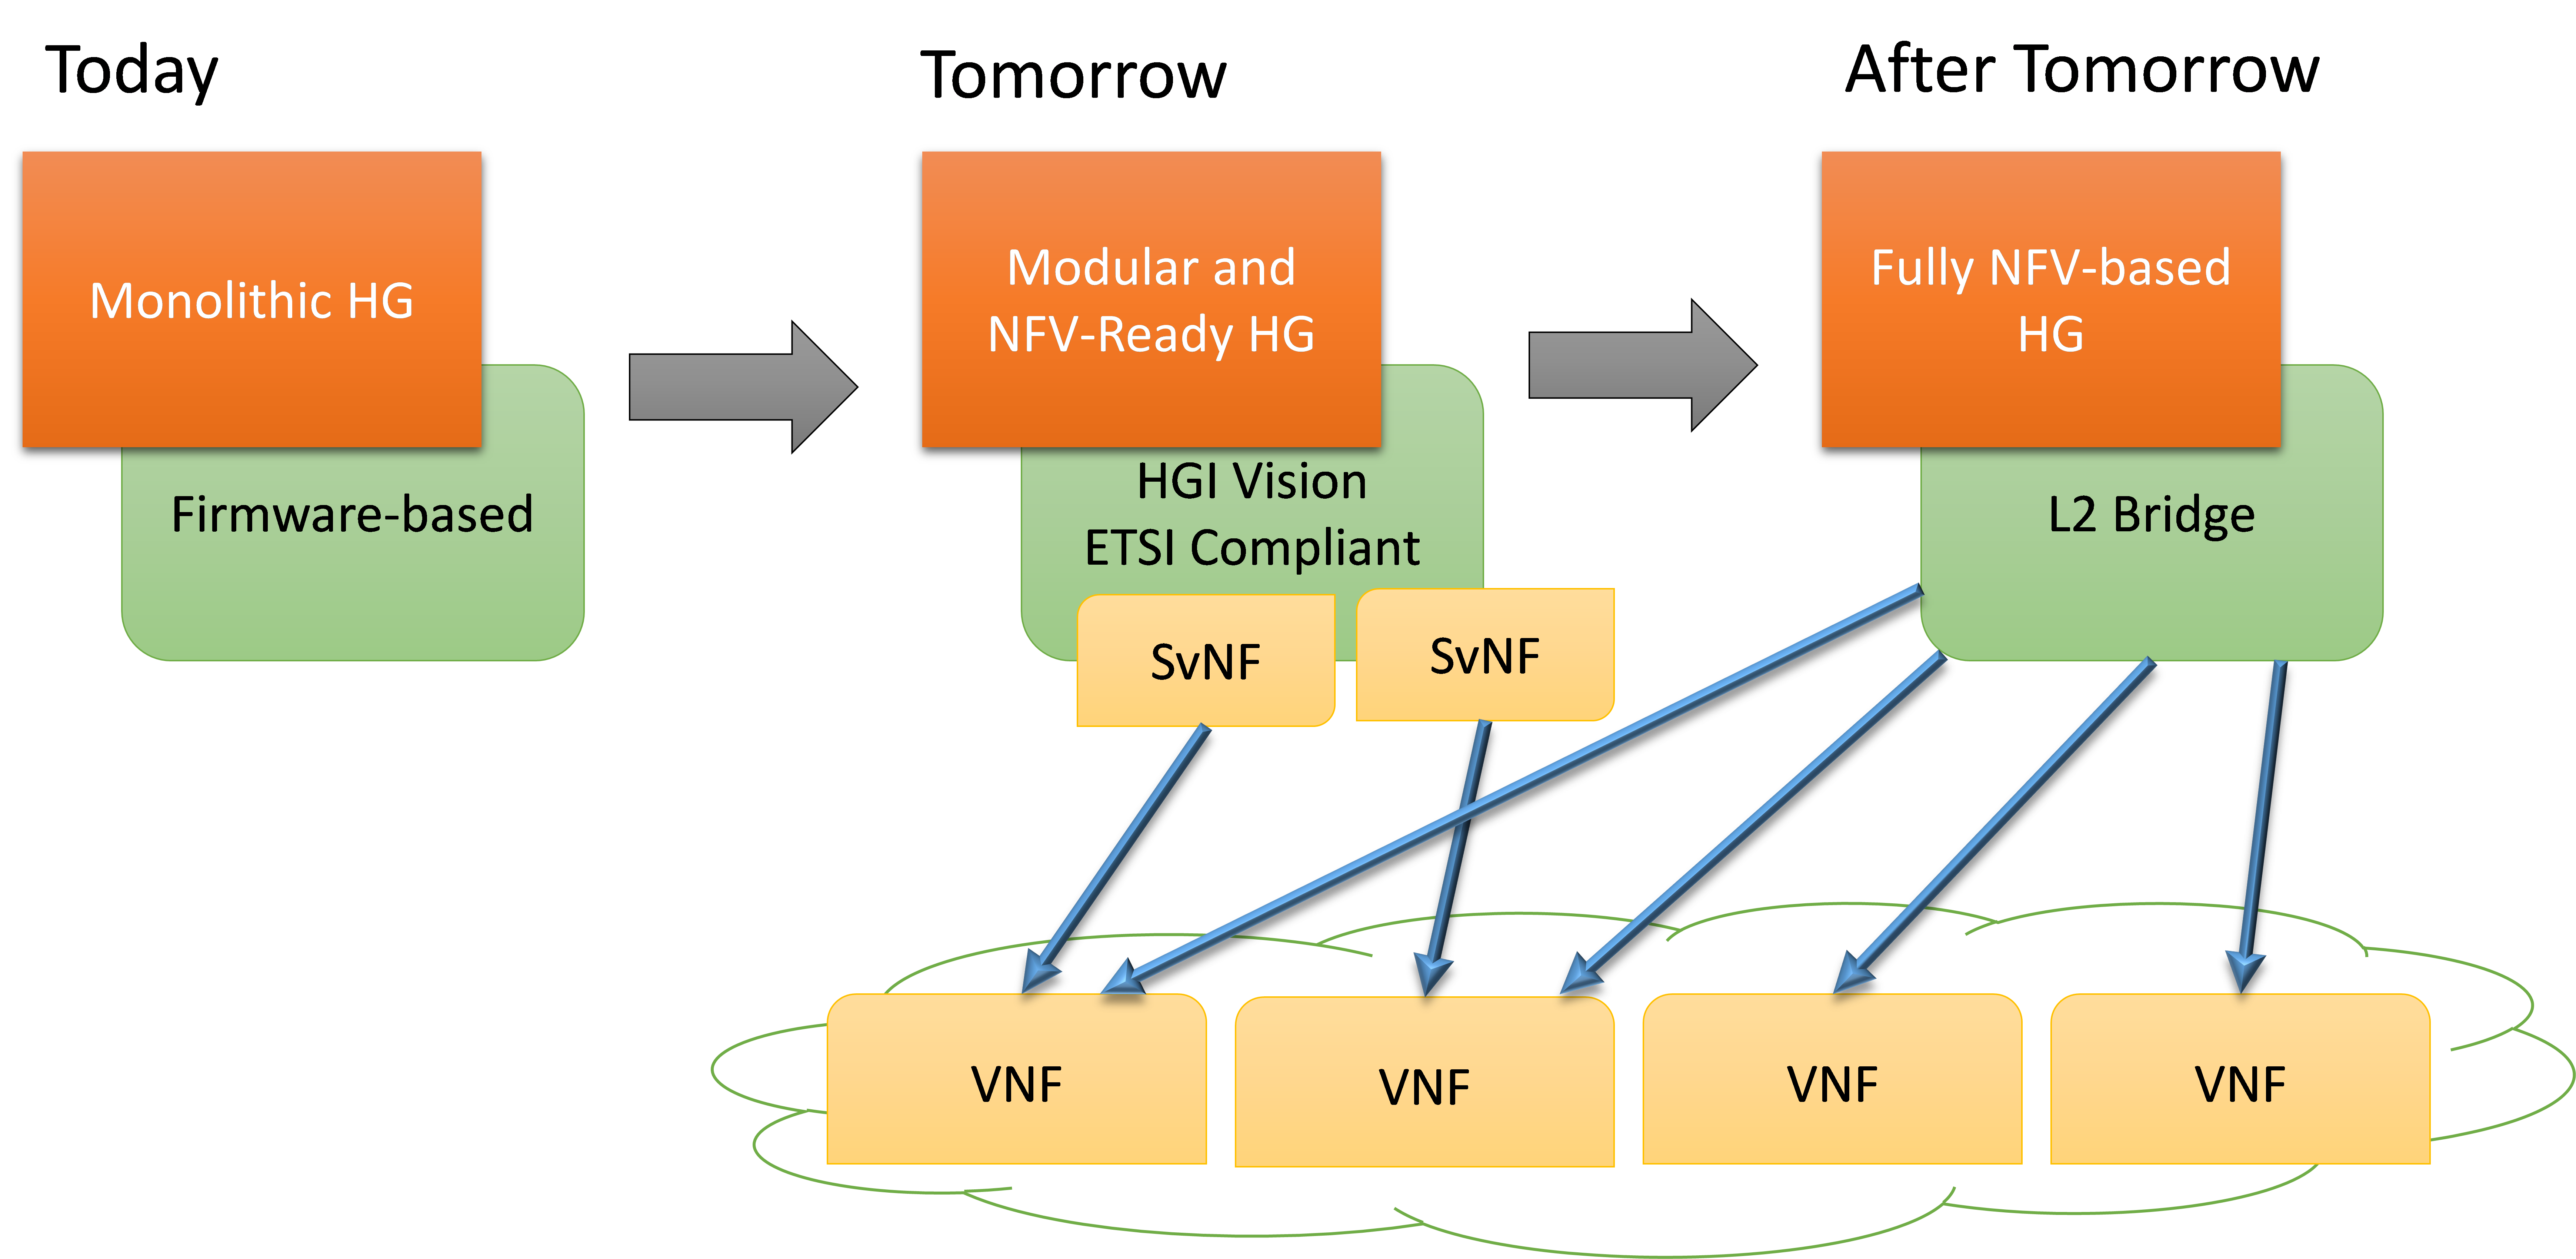
\includegraphics[width=0.45\textwidth,natwidth=6955,natheight=3398]{fig/vhgMigrationPath.png}
  \end{center}
  \caption{ Migration path from Modular to Virtual HG.
    \label{fig:migration}
  }
\end{figure}


\subsection{The NFV ready Modular HG}
We propose an alternative migration path where vNFs collaborate with modular gateways.
Figure~\ref{fig:migration} presents a Modular HG with \textit{"Surrogate vNF"} (SvNF) deployed on the device.
A SvNF is an OSGi bundle that acts like a regular module from the HG standpoint, except that it delegates any significant operation to a vNF.

SvNF modules [N6][n7]can be aware of SP access network capabilities to support vNFs, so they can be registered in the HG OSGi execution environment only if they are supported by the underlying network.
For example, if the gateway cannot find any suitable vNF in a predefined SP point of presence (POP) list, it will fall back on legacy mode and keep using the native functionality instead of the virtualized one.

The key role played by the couple SvNF+vNF in the migration path is that the vNF part is used on both the OSGi modular gateway scenario and on the L2 bridge scenario.
This approach helps the SP stabilising its vNF before gradually migrating all its customers to the full vNF solution while securing investments made on developing the vNF.
 
\subsection{Concept and feasibility}
To demonstrate the feasibility of a modular and NFV-ready HG, we realized a proof of concept (POC).
In order for this POC to be highly relevant, we had to consider the best possible Network Functions to be virtualised.
We could have focused on simple functions such as DHCP or NAT but since they are not difficult tasks to be processed, the added-value of virtualizing them appears limited. We thus decided to highlight the advantages of our proposal by deploying a new type of SvNF+vNF related to video distribution that would leverage the End-User's Quality of Experience related to video consumption and enhance network performances at the same time. Such a function can be introduced into a modular OSGi HG and its execution would definitely be efficient as a vNF, due to the heavy video processing tasks it involves. It is expected that IP video traffic will reach almost 80% of all consumer Internet traffic in 2018 [CISCO forecast white paper: http://www.cisco.com/c/en/us/solutions/collateral/service-provider/ip-ngn-ip-next-generation-network/white_paper_c11-481360.html], therefore it seems important to focus on how new solutions, such as NFV, could not only cope with this but especially enhance the delivery of such data.

\begin{figure*}
	
	\center

	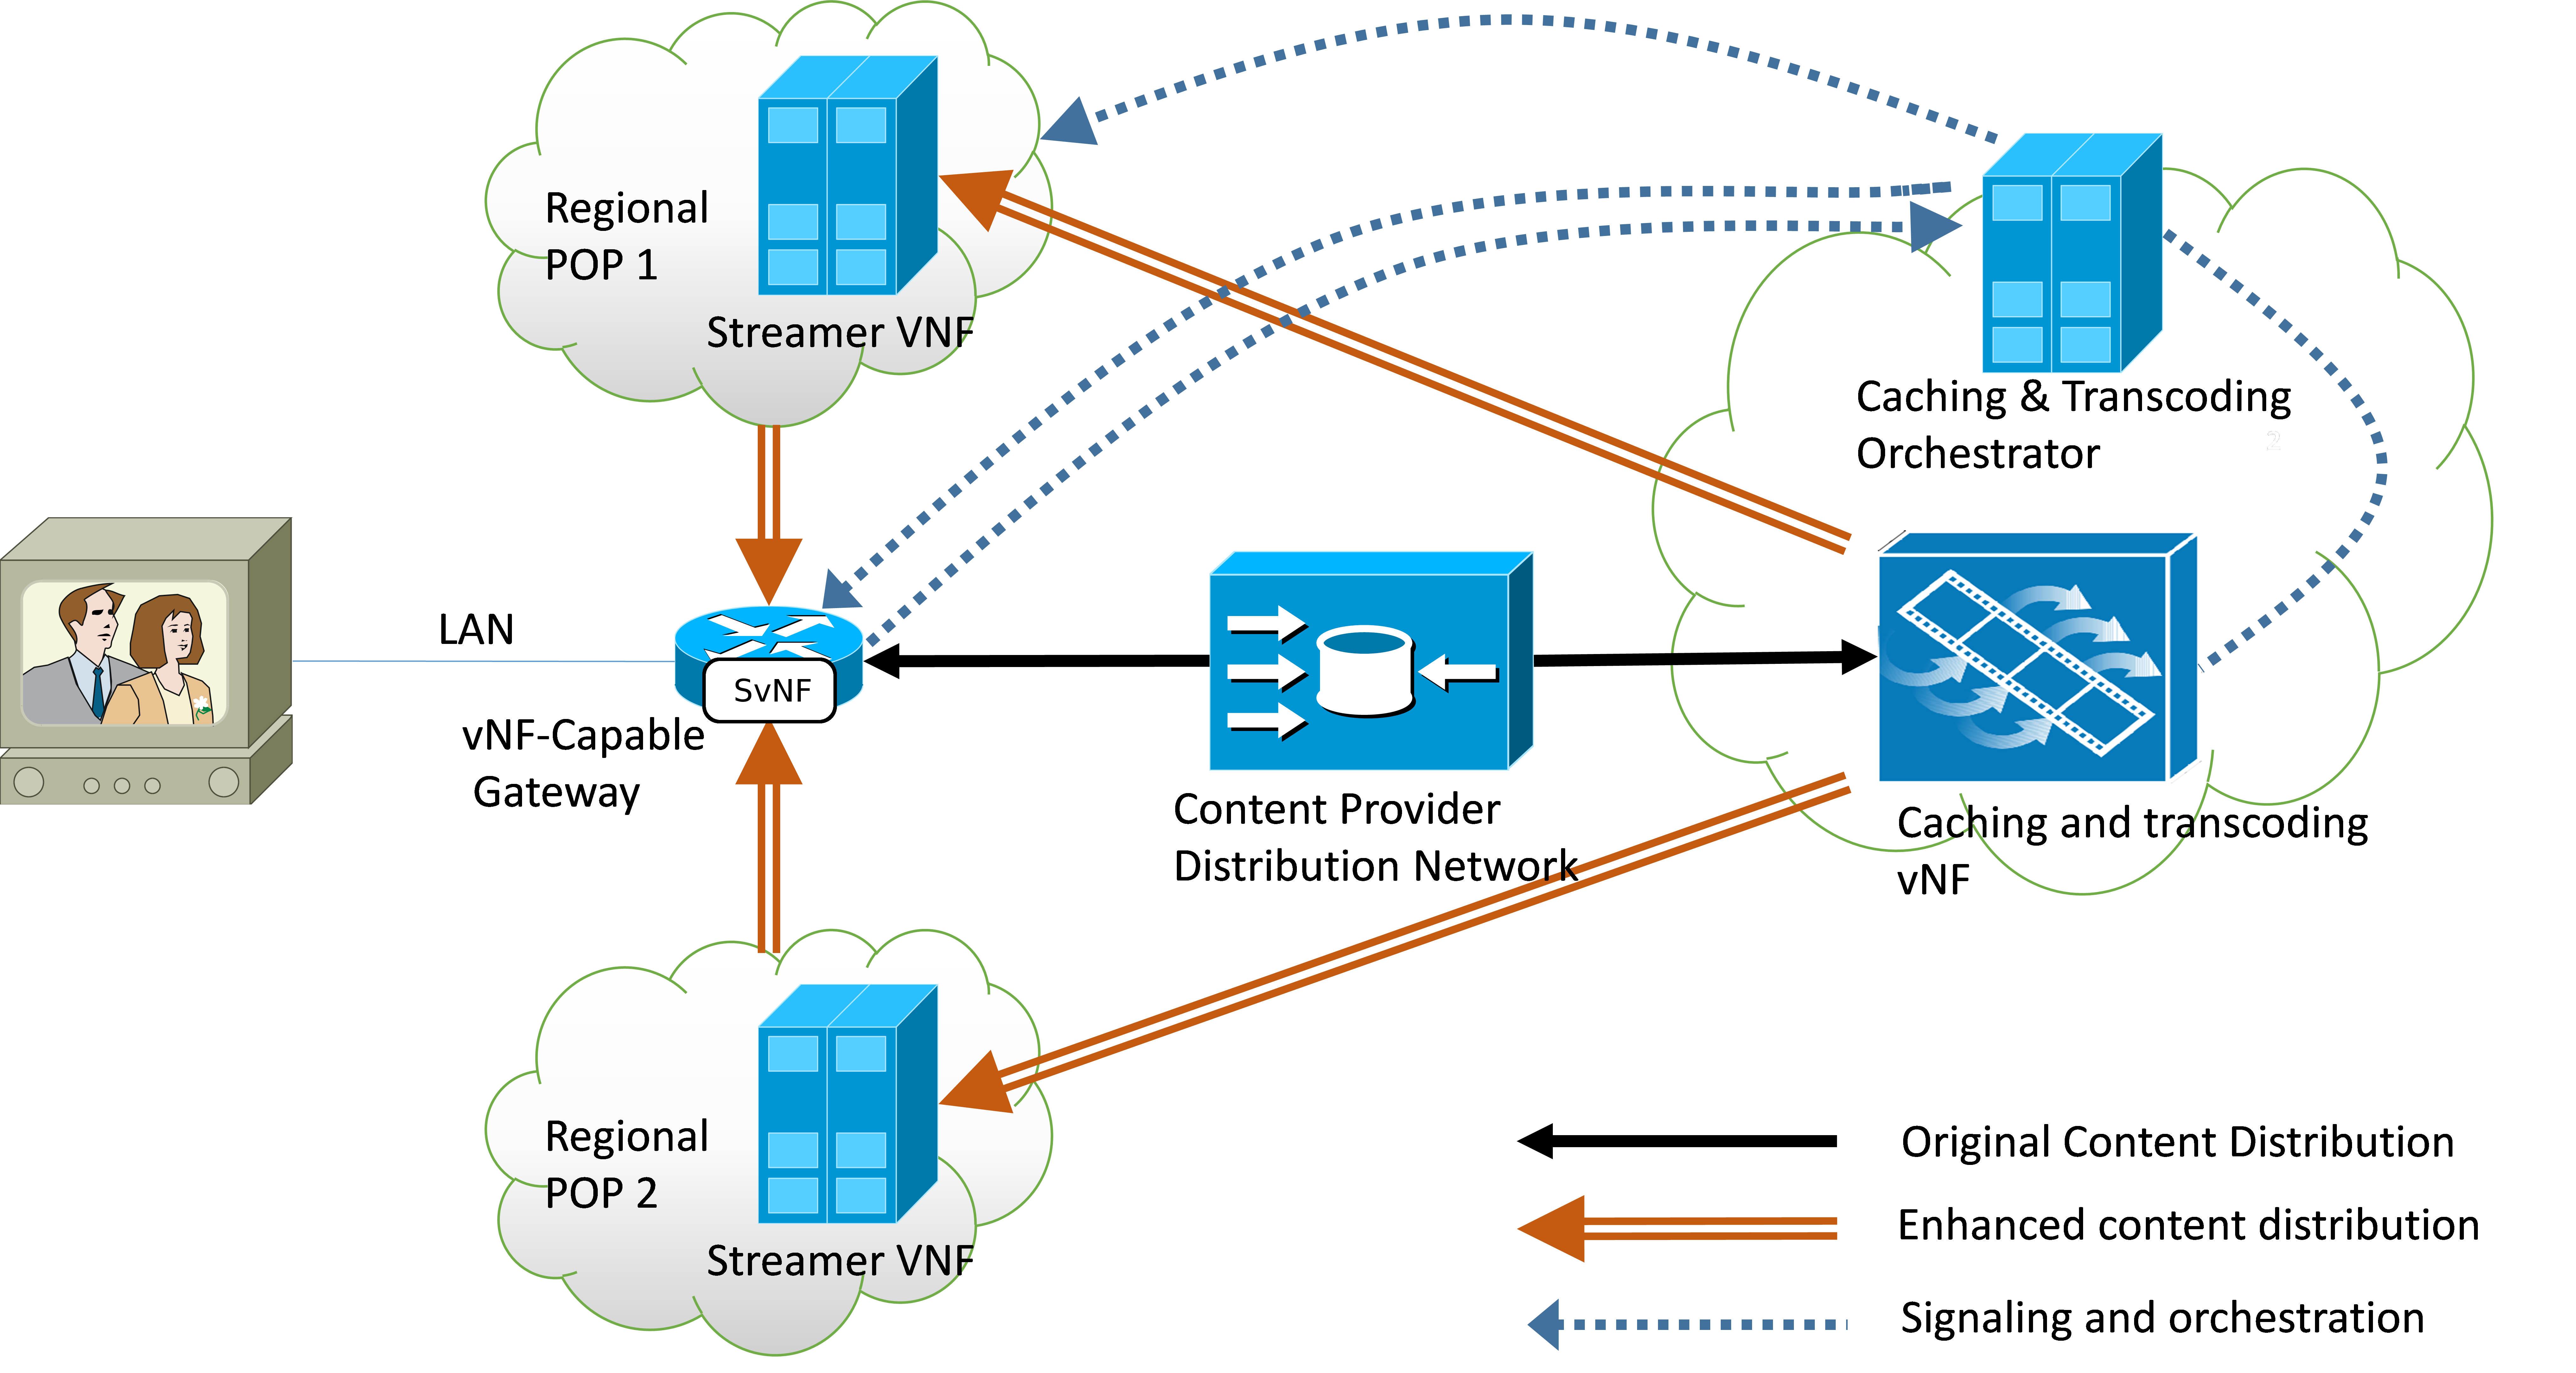
\includegraphics[width=0.90\textwidth,natwidth=8132,natheight=4335]{fig/highleveldesign.png}
	\caption{ High level design
    \label{fig:hld}
    }

\end{figure*}


The use case considered consists of an End User consuming media from his Set-Top Box, linked to his HG (the two devices are more and more often combined into one).
Video streams of a VOD or IPTV service are transferred from the content provider distribution network (which may or may not include Content Delivery Networks - CDNs) to the TV and cross the modular OSGi Gateway.
Figure~\ref{fig:hld} depicts the design of the system and the use case steps. 
   
The figure presents the interactions between CP, SP and EU for a classical video streaming use case.
In the original content distribution model, content is stream from the content provider network to the user gateway.
Classic deployment scenario involve the use of content distribution network to offload the CP main server.
CDN nodes are often collocated with internet exchange points (IXP) which present the advantage of being located relatively close of the EU.
Our use case however, presents an alternative model where the content is cached in regional POP managed by SP (also called micro-data centers located at the edge of the network) and exposed for streaming by a vNF.
Caching and encoding orchestrator manages configuration deployments of the SvNF on the gateways, the provisioning of regional POPs, as well as the caching and transcoding vNF.

The SvNF module deployed on the HG works as a HTTP proxy.
When it receives a request for a file or a response from a server, it analyses them using a set of rules deployed on the HG by the Caching and Transcoding Orchestrator through the "Caching Control and Configuration Channel".
Depending on the result several scenarios can occur.
Content could be available only in the CP network or an enhanced version could be cached by the system into a close regional POP.
Let's consider the three possible scenarios.
For the three possible scenario, the steps 1 and 2 are the same. 

\paragraph{Step1}EU requests the content from the vNF-Capable Gateway. 
\paragraph{Step 2}
The vNF-Capable Gateway analyses the video format, and checks it is technically compatible with the system (e.g. a supported video codec and supported delivery method).
If it is compatible, we continue to scenario 2, otherwise, we proceed with scenario 1.

\subsubsection*{Scenario 1: no operation scenario}

In this scenario, the content consumed by the user is not eligible to the enhancements brought by the system.
After the gateway has analysed the request, it if forwarded to its original destination.

\paragraph{Step 3}The content is then directly consumed by the End-User from the Content Provider Delivery Network.
This is the common case, as it is performed today.
The HG does not bring any added value to the consumption of video streams.
It just lets the content pass through it.

In this case, the SvNF creates an overhead on the gateway without bringing additional value to the user.
This overhead needs to be measured in order to know if it would penalize the user experience (and in which extent).

\subsubsection*{Scenario 2: Cache hit scenario}

Let's now consider that the content has been processed by the system and is made available in regional POPs.
Those are part of the NVF infrastructure, and handle mostly storage and delivery of content.
They are managed by SP and can be collocated with existing O-CDNs (operator-managed CDN).
The Caching and Transcoding Orchestrator has configured SvNF so that the HG redirects the user request to a Streamer vNF.
Hopefully, those vNFs are deployed in regional POPs and provisioned in a way that network performances are enhanced with respect to the original Content Provider network.
The main value compared with the CDN approach is that content has been processed by the system and a "better version" of it is made available to the user through QoE enhancing techniques we will describe latter in (reference).

We can also consider that by leveraging the existing SP network, the approach can provide POPs that are much closer from the EU than in the CDN scenario.
This is a great way for the CP to generate extra revenue from its network.	

\subsubsection*{Scenario 3: Cache miss scenario}

Finally, the last scenario is the one where the content is eligible for caching and transcoding but no cached version is yet available to the vHG from where the request has been made[N15][n16].
In this case the cache is missed and the content is retrieved from the CP.

If the content only resides on the CP distribution network, user request is left untouched and media is consumed from there.
However, under the hood, SvNF has analysed both request and response and has checked if media was eligible for caching and transcoding.
The decision is made taking into account several properties on the HTTP resources like server domain, file type, file size and any relevant HTTP headers.
When an eligible content is found, the SvNF informs the Caching and Transcoding Orchestrator by sending a caching request.
Caching and Transcoding Orchestrator takes the decision to perform caching and transcoding on the content based on several criteria ranging from Context and User Intelligence (which has been proven in [23] to improve the performance of content delivery), to business negotiation between Content Provider and service Provider.

If the Caching and Transcoding Orchestrator decides to process the content, it informs the Caching and Transcoding vNF which in turn is in charge of downloading the content from the content provider and processing the content.
Once processed, the Caching and Transcoding Orchestrator provision streamer vNF in regional POPs according to the demand.
We develop on the specific operations carried out by the Caching and Transcoding vNF in (reference).

Once the content is deployed in selected POPs, the configuration is published to vHGs, allowing future requests to be routed to vNF streamers.

Otherwise, if the content is already available in other POPs in the system, the caching and transcoding orchestrator may reconsider its provisionning decisions by deploying the content in additional POPs in order to match a certain SLA.
This operation should be carried out with the help of the underlying NFV platform, like the T-NOVA project.

\subsection{In-network processing benefits for CP and SP}
The NFV approach allows us to process data directly in the network.
For our use case, it means that we can apply arbitrary modification to a video with a view to optimize the delivery with respect to a specific technical or business objective.
For example, targeted ads can be added to the video by the SP with a view to increase profit, QOE can be increased by transcoding the content into a specific format which has this property.
The fact that we are able to transform the content directly into the network[N19] is a big advantage in term of flexibility and convenience of administration for CP and SP.

One other striking features of NFV is its ability to dynamically provision network functions according to simple business requirements expressed as Service Layer Agreements (SLA).
To fine-tune orchestration policy of the system, SP could set a target of 10Mps in the 7pm-10pm time slot for its user toward a specific VOD website.
Once the vNF is configured with those targets, Caching and Transcoding Orchestrator has to do its best to respect the SLA by using NFV infrastructure metrics (CPU, IO, Memory) but also specific application metrics.
Thanks to the key roles played by the HG, our solution offers the possibility to collect metrics at the user level and hence using a Collective Intelligence approach to optimize system operation according to SLA targets. 

Collective intelligence data is collected thanks to caching requests emitted by vHG.
The system gathers data which reflect video consumption patterns on a per-user basis, like user average bandwidth, hourly consumption patterns, and consumption habits.
Let's imagine a particular user watch HBO's Game of Thrones every Monday evening on his Ipad which support Apple's HTTP Live Streaming (HLS) on a T1 connection.
If this pattern is widespread amongst users, the Caching and Transcoding Orchestrator can assign a higher priority on the transcoding of the HD HLS version of the popular TV show and assuring the correct provisionning on selected regional POPs.

This approach allows CP to broadcast its content in cooperation with SP NVF network with limited technical interaction.
Indeed, expressing contractual SLA target is enough for the CP to deploy its content, as the SP's vNF becomes responsible for determining (1) which content to cache (2) which enhancements to bring to the content and (3) where to cache the content.


\section{Results \label{sec:results}}

\begin{table*}
	\centering
	\begin{tabular}{|p{0.10\textwidth}|p{0.35\textwidth}||p{0.10\textwidth}|p{0.10\textwidth}|p{0.10\textwidth}|p{0.10\textwidth}|}
		\hline
		\multirow{2}{0.10\textwidth}{Settings} & \multirow{2}{0.35\textwidth}{Detail of the network topology and software involved}   & Video Download Throughput from NAS & Video Download Throughput from Internet CDN      & Web Browsing Throughput from NAS & Web Browsing Throughput from Internet CDN \\ \cline{3-6}
		 & & \multicolumn{2}{m{0.20\textwidth}|}{5 threads continuously downloading a 20 Mb video file. 1000 times} & \multicolumn{2}{m{0.20\textwidth}|}{5 threads continuously downloading 172 files of 16kb. 1000 times}\\\hline\hline
		Direct Connection & Test machine connected directly to Internet & 191.5 ipm \footnote{items per minute} & tbd & 208.2 ipm & 58.5 ipm \\\hline
		IP Relay  & Test machine connected on the gateway with IP relay & 184.5 ipm & tbd & 200.3 ipm & 58.5ipm\\\hline
		\multirow{3}{0.10\textwidth}{Squid3 with cache disabled} & \multirow{3}{0.35\textwidth}{
		Test machine connected to the gateway. Squid3 with cache disabled} &185.0 ipm & \multirow{3}{*}{tbd} & 192.5 ipm & 55.2 ipm \\
		 & & 25\% CPU & & 27\% CPU & 12\% CPU \\
		 & & 1.5\% Mem & & 1.5\% Mem & 1.5\% Mem \\\hline
		
		\multirow{3}{0.10\textwidth}{Java Proxy without rules} & \multirow{3}{0.35\textwidth}{
		Test machine connected to the gateway,OSGi HTTP proxy launched on the gateway with no rules deployed} &184.d ipm ipm & \multirow{3}{*}{tbd} & 165.d ipm & 59.d ipm \\
		 & & 39\% CPU & & 40\% CPU & 20\% CPU \\
		 & & 2.5\% Mem & & 2.5\% Mem & 2.5\% Mem \\\hline
		 
		 \multirow{3}{0.10\textwidth}{Java Proxy with 10000 "rules"} & \multirow{3}{0.35\textwidth}{
		Test machine connected to the gateway, OSGi HTTP proxy launched on the gateway with 10.000 "rules" deployed} &178.3 ipm & \multirow{3}{*}{tbd} & 162.d ipm & 57.d ipm \\
		 & & 45\% CPU & & 49\% CPU & 24\% CPU \\
		 & & 2.5\% Mem & & 2.5\% Mem & 2.5\% Mem \\\hline
                                                
	\end{tabular}
	\caption{
	OSGi HTTP proxy performance comparison
	\label{tab:perf-comparison}
	}
	
\end{table*}


From what we saw in Section~\ref{sec:migrating}, the main aspects we need to focus on to validate our approaches are:
\begin{itemize}
	\item Is it feasible to have a NFV-ready modular OSGi HG, with a SvNF+vNF related to video distribution?
	\item What is the overhead associated with the proposed HG architecture composed of an OSGi bundle acting as a HTTP proxy?
	\item What are the benefits of a NFV-ready modular HG in terms of (1) End-User QoE and (2) Network performance considering the video delivery use case?
\end{itemize}


\subsection{Results}
  \subsubsection{Testbed}
   We used commodity hardware along with 100 Mb Ethernet network.
   As software, Ubuntu 14.04 for hypervisors and Debian 7 for the VM and gateway were used.
   Details are represented in Figure 5. 6 Workers were started throughout the experiment.
  \subsubsection{NFV Infrastrucre}
   Our work is supported by the European FP7 T-NOVA project which aims at providing a NFV infrastructure based on ETSI standards.
   For the time being, we simulated this infrastructure by using virtual machines deployed on a commodity server.
   We used QEMU/KVM for the virtualization part.
  \subsubsection{Remote resources}
   For performance assessments, we made sure that remote resources accessed through the Internet would be deployed in the most stable environment possible.
   This helped us ruling out possible network noise during our test procedures
   
   We used a local public Content Delivery Network provider to deploy video resources, since deploying them on a regular web server came out being too prone to network errors and latency variations.
  \subsubsection{Testing Methodology and Goals}
JMeter\footnote{http://jmeter.apache.org} was used to capture the network metrics of our solution.
It allowed us to create agents and make them perform standard HTTP and report on specific performances metrics.    
Among the metrics that we collected, we decided to analyse the throughput which is defined by JMeter to be the number of resources downloaded by minutes.
We used 2 different resources for our experiment.
First, we considered a 20 Mb video file, then a single HTML page which links to several other static resources like Javascript files, CSS or images. 
   The throughput metric reflects several key aspects for performance:
   \begin{itemize}
   \item The latency, which is the time elapsed between the end of the query and the beginning of the response
	\item The download time, which is the time between the beginning and the end of the response.
   \end{itemize}
We decided that the best and simplest way to represent the impact of the SvNF on the performance was to measure the throughput for different scenario. In the first scenario, a 20 Mb video file is downloaded, for the second scenario, a HTML page is downloaded along with 171 other attached resources of average size 16 kb. It is clear that the first scenario result will reflect the impact on the download time while the other will be much more sensitive to latency, due to the amount of smaller resources to download.
We developed the following modules
\begin{itemize}
\item An OSGi Bundle deployed on the HG
\item A Server part which is divided into 
\begin{itemize}
\item Central Caching Orchestration Agent
\item Streamers vNF
\item Workers vNF
\end{itemize}

\end{itemize}	

% Please add the following required packages to your document preamble:





\section{Conclusion and future work \label{sec:conclusion}}

conclusion


\section*{Acknowledgments}
The work in this paper has been performed within the T-NOVA project. T-NOVA is an Integrated Project co-funded by the European Commission / 7th Framework Program, Grant Agreement no. 619520.
\bibliographystyle{IEEEtran}
\bibliography{vnf}





% that's all folks
\end{document}


